\chapter{Introduction}
TODO: 
Definições de grafo, grafos cúbicos,homomorfismo e profas auxiliadas por computador 

SENTENCE SUGGESTION: whenever possible, we illustrate definitions and methods with python based algorithms

\section{Graphs}

Graphs are mathematical structures first described by \emph{Euler} to solve the \emph{Seven Bridges of Königsberg} problem - TODO add citation -. 
Are used to model different gammas of real world problem including deadlock detection, shortest paths, package routing, among numerous others. 

A Graph $G$ can be defined as a set of vertices $V(G) \subset \mathbb{N}$ and edges $E(G) \subseteq [V^2]$. 
For every $\{u, v\} \in E(G)$, we call $u$ and $v$ neighbours. 
We say that the neighborhood $N_G(v)$ of a vertex $v \in V(g)$ are neighbors of $v$ in $G$ and the degree $d_G(v)$ as $|N_G(v)|$.
A graph for which the degree of every vertex has the same value $r$ is a $r$-$regular$ graph and, specifically, for $r=3$ a \emph{cubic} graph.
A \emph{complete graph} is a $(n-1)$-$regular$ graph where $n=|V(G)|$.
$K_n$ is the complete graph of size $n$.

We say that the graph $G'$ is a \emph{subgraph} of the graph $G$ if and only if $V(G') \subset V(G)$ and $E(G') \subset E(G)$, we, then, can write $G' \subset G$. 
A \emph{path} $P$ in a graph $G$ is a sequence of vertices $(x_1, \dots, x_k)$ such that, for every $1 \leq i < k$, $\{ x_i, x_{i+1} \} \in E(G)$. 
If all vertices in $P$ are distinct and $\{ x_1, x_k \} \in E(G)$, we call it a \emph{cycle} with size $k$.
$G$ is \emph{connected}, if for every pair of vertices $u$ and $v$ in $G$, there is a path starting in $u$ and ending in $v$.

TODO: [n]

$C_n$ is a graph with $n$ vertices such that there is cycle $P=(x_1, \dots, x_n)$ and $E(C_n) =\{ \{x_i,x_{i+1}\} | 1 \leq i < n \} \cup \{\{x_1,x_n\}\}$. 
It's easy to that $K_3$ and $C_3$ are the same graph show on Figure \ref{fig:k3}.
The \emph{girth} $g$ of Graph $G$ is length of the the shortest cycle which is a subgraph of $G$.
If there is no such cycle, $G$ is \emph{acyclic} with girth $g= \infty$.

We say that a graph is a \emph{tree} if it is acyclic and connected. Vertices in a tree are a called leafs nodes if their degree is one and internal otherwise.  

For any graphs $G_1$ and $G_2$, a homomorphism is a function $h \colon G_1 \to G_2$ such that $\{h(u), h(v)\} \in E(G_2)$ for every edge $\{u, v\} \in E(G_1)$. 

Given graphs \(G\) and \(H\), an \emph{homomorphism} from \(G\) to \(H\)
is a function \(h\colon V(G) \to V(H)\) for which \(h(x)h(y)\in E(H)\) whenever \(xy\in E(G)\).
For ease of notation, in this case, we write \(h\colon G \to H\).


 \begin{figure}
    \centering
    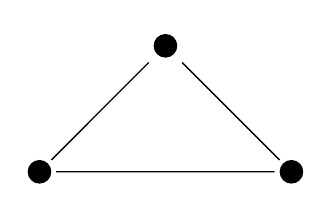
\begin{tikzpicture}[node distance=2cm,scale = .8]
% Vértices
\tikzset{black vertex/.style={circle,draw,minimum size=1mm,inner sep=0pt,outer sep=2pt,fill=black, color=black}}

  \node (0) at (0,0) {0};
  \node[black vertex] () at (0,0) {0};
  \node[black vertex] (1) at (2,-2) {1};
  \node[black vertex] (2) at (-2,-2) {2};

% \draw[line width = .5pt] (0) -- (1) (2) -- (3) (4) -- (5) (6) -- (7) (8) -- (9) (10) -- (11) (12) -- (13) (14) -- (15);

\draw[line width = .5pt] (0) -- (1) (0) -- (2) (1) -- (2) ;

\end{tikzpicture}
    \caption{$K_3$}
    \label{fig:k3}
\end{figure}



\section{Computer-assisted proofs}
